\chapter{METODOLOGI}

\section{DESKRIPSI SISTEM}

\subsection{Arsitektur Sistem}

\begin{figure} [ht] \centering
  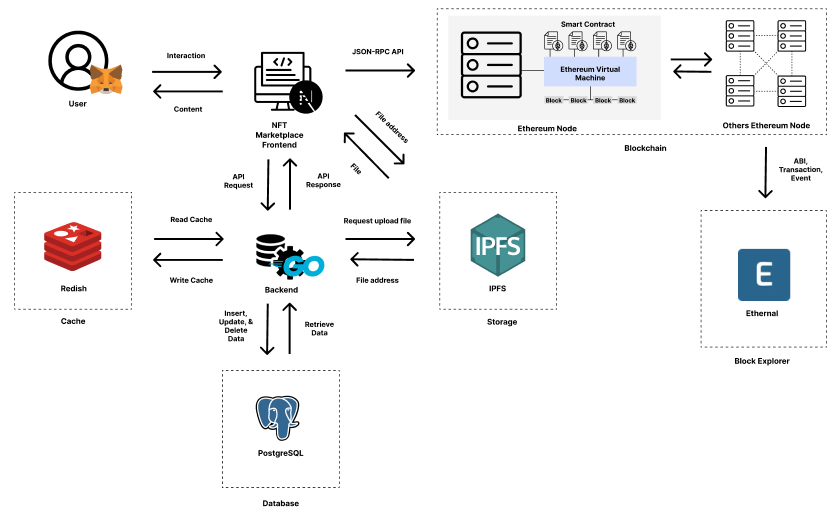
\includegraphics[scale=0.45]{gambar/img-architecture.png}
  \caption{Arsitektur NFT \emph{Marketplace}}
  \label{fig:Architecture}
\end{figure}

Dalam pengembangan suatu \emph{NFT Marketplace} ini diperlukan suatu arsitektur supaya sistem yang dikembangkan dapat bekerja sesuai dengan yang diharapkan. Pada \emph{NFT Marketplace} ini terdapat 2 \emph{role user} yaitu \emph{owner} yang merupakan pemilik dari suatu \emph{token} dan \emph{user} yang merupakan pihak yang memiliki akses terbatas terhadap suatu token dalam waktu yang telah ditentukan. Untuk dapat mengakses \emph{NFT Martketplace} baik \emph{owner} ataupun \emph{user} harus terhubung menggunakan \emph{wallet} dalam berinteraksi. 

Pengguna yang sudah terhubung dengan \emph{wallet} dapat berinteraksi dengan \emph{front end} aplikasi \emph{NFT Marketplace}. \emph{Frontend} akan terhungu dengan aplikasi \emph{backend} ketika pengguna melakukan \emph{Minting} dimana prosesnya pengguna mengunggah aset digital yang dimiliki dan diunggah ke \emph{IPFS} melakukan aplikasi \emph{backend} dan akan mengembalikan \emph{Content Identifier} (CID). \emph{CID} merupakan sebuah \emph{address} file dalam \emph{IPFS} yang digunakan untuk mengakses file tersebut. \emph{CID} yang diperoleh kemudian akan diunggah ke jaringan \emph{blockchain} dan menjadi suatu \emph{token}. Data-data mengenai \emph{NFT} yang tersedia dapat langsung diperoleh \emph{frontend} melalui \emph{smart contract} pada \emph{blockchain}. Selain itu dalam praktiknya aplikasi \emph{backend} juga akan menyediakan data-data seperti harga token melalui API yang disediakan oleh CoinMarketCap. Untuk memperoleh data mengenai estimasi \emph{gas fee} yang diperlukan aplikasi \emph{backend} juga terhubung dengan \emph{API ETH Gas Station}.

\subsection{\emph{Flow} Pembelian Token}

% Contoh input gambar dengan format *.jpg
\begin{figure} [H] \centering
  % Nama dari file gambar yang diinputkan
  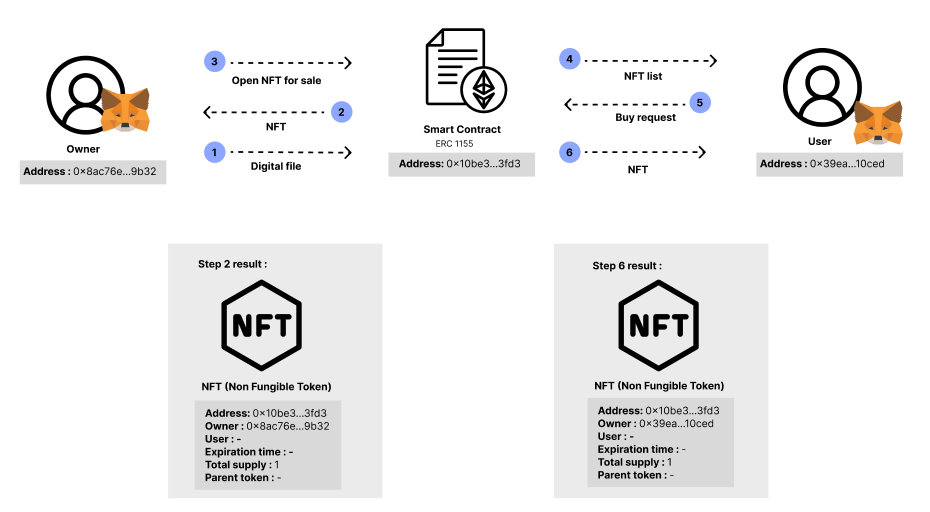
\includegraphics[scale=0.45]{gambar/img-nft-buy.png}
  % Keterangan gambar yang diinputkan
  \caption{\emph{Flow} pembelian \emph{Token}}
  % Label referensi dari gambar yang diinputkan
  \label{fig:Buy}
\end{figure}

Pembelian pada \emph{smart contract} yang akan dikembangkan menggunakan fungsi dari \emph{interface} \emph{ERC-1155}. \emph{Interface} ini memungkinkan \emph{token fungible} dan \emph{non-fungible} diperjual belikan dalam satu kontrak. Hal ini dimungkinkan dengan adanya penambahan properti \emph{supply} pada \emph{token}. Jika \emph{supply token} bernilai 1 maka \emph{token} tersebut akan diperlakukan sebagai \emph{NFT} sebaliknya maka token akan diperlakukan layaknya \emph{fungible token}.  

\subsection{\emph{Flow} Penyewaan NFT}

\begin{figure} [H] \centering
  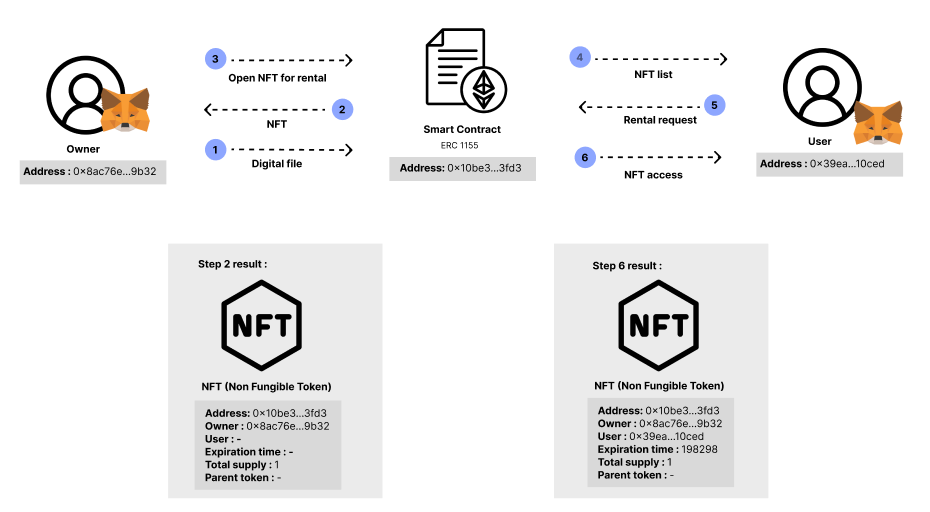
\includegraphics[scale=0.45]{gambar/img-nft-rental.png}
  \caption{\emph{Flow} penyewaan \emph{NFT}}
  \label{fig:Rental}
\end{figure}

Pemilik \emph{token} dapat menyewakan \emph{token} yang dimiliki kepada pengguna lain untuk memperoleh keuntungan selain melakukan penjual. Hal ini dimungkinan dengan adanya pemisahan \emph{role owner} dan \emph{user} pada \emph{token}. \emph{Owner} adalah pemilik token yang memiliki seluruh akses terhadap \emph{token} sedangkan \emph{user} adalah pihak yang memiliki akses terbatas terhadap token dan juga dibatasi dalam periode yang telah ditentukan.

\subsection{\emph{Flow} Pembagian Kepemilikan NFT}

% Contoh input gambar dengan format *.jpg
\begin{figure} [H] \centering
  % Nama dari file gambar yang diinputkan
  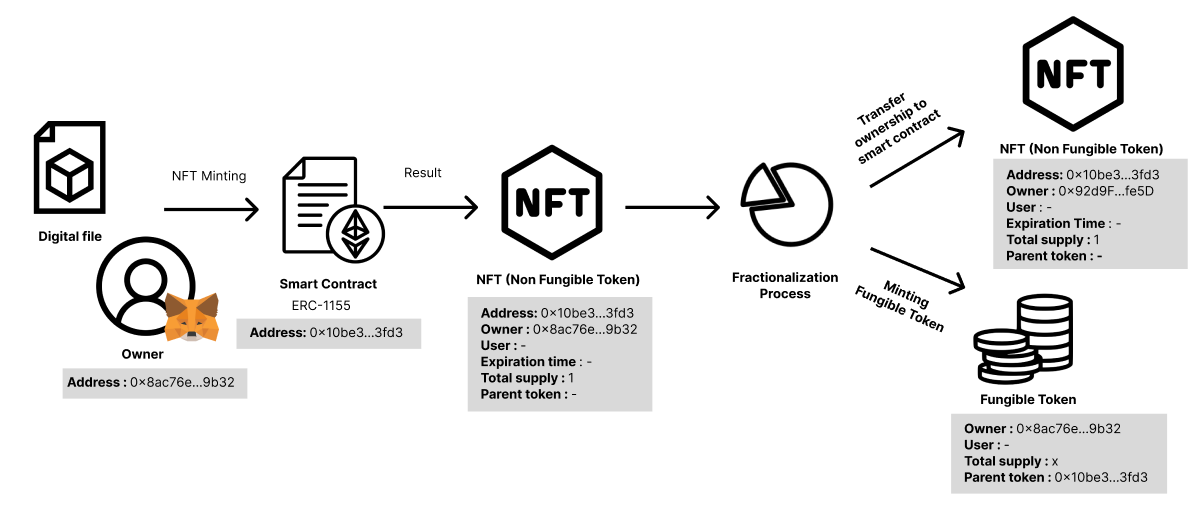
\includegraphics[scale=0.35]{gambar/img-fractional-nft.png}
  % Keterangan gambar yang diinputkan
  \caption{\emph{Flow} pembagian kepemilikan NFT}
  % Label referensi dari gambar yang diinputkan
  \label{fig:Fractional}
\end{figure}

Pembagian kepemilikan \emph{NFT} dilakukan melalui proses \emph{fractionalization}. Proses ini membuat \emph{NFT} ditransfer kepemilikannya ke pemilik \emph{smart contract}. Selain itu \emph{fungible token} dengan jumlah yang telah ditentukan akan di-\emph{minting}. \emph{Fungible token} ini lah yang akan merepresentasikan kepemilikan atasnya atas \emph{Parent Token}. Jika \emph{NFT} disewakan maka seluruh pemilik \emph{token fraction} akan memperoleh keuntungan sesuai dengan jumlah kepemilikannya atas \emph{token fraction}.

\subsection{\emph{Metadata}}

Berdasarkan \emph{interface} ERC-721 setiap NFT memiliki \emph{metadata}. \emph{Metadata} sendiri adalah data yang menyusun konten dari NFT tersebut dan biasanya dinyatakan dalam format JavaScript Object Notation (JSON). Data yang disimpan dalam \emph{metadata} biasanya meliputi nama, deskripsi, tautan ke gambar yang dapat disesuaikan dengan kebutuhan aplikasi desentral yang dibangun. Untuk menstandarisasi NFT maka \emph{metadata} yang ditetapkan pada \emph{project} NFT \emph{Marketplace} ini adalah sebagai berikut

\begin{figure} [H] \centering
  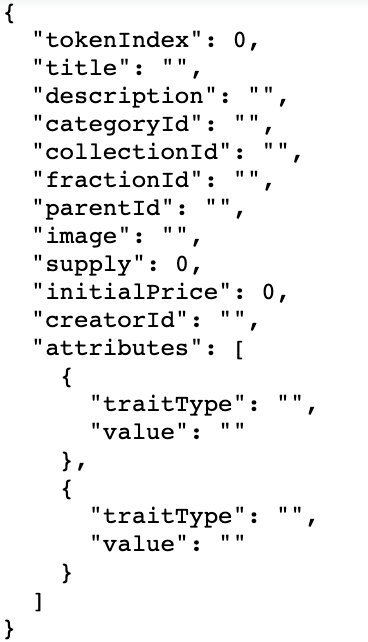
\includegraphics[height=7cm]{gambar/img-metadata.png}
  \caption{Metadata NFT}
  \label{fig:MetadataNFT}
\end{figure}

Atribut pada metadata di atas merupakan data-data yang terikat dengan \emph{NFT} yang dapat disesuaikan dengan kebutuhan masing-masing platform dimana data ini juga di simpan dalam format \emph{JSON (Javascript Object Notation)} berupa \emph{Array} dengan \emph{elemen object}. Setiap \emph{Object} tersebut memiliki dua \emph{field} yaitu \emph{traitType} yang merupakan nama data dan \emph{value} merupakan nilai dari data tersebut. Dengan adanya \emph{Attributes} membuat \emph{NFT} dapat \emph{compatible} dengan berbagai \emph{platform} lain.

\subsection{Integrasi Platform Lain}

Integrasi dengan platform lain menjadi hal yang penting dikarenakan \emph{NFT Marketplace} yang ingin dikembangkan diperuntukan supaya dapat digunakan oleh platform lain yang mengusung konsep \emph{metaverse}. Supaya \emph{platform} lain dapat terintegrasi dengan \emph{NFT Marketplace} yang dikembangkan terdapat \emph{API (Aplication Programming Interface)} yang disediakan. Langkah-langkah sebelum integrasi melalui \emph{API} adalah \emph{platform} tersebut perlu menyediakan fitur autentikasi melalui \emph{Wallet} atau menghubungkannya dan juga melakukan \emph{minting} melalui \emph{NFT Marketplace}. Berikut merupakan diagram tahapan dalam integrasi

\subsection{\emph{Minting}}

Hal pertama yang perlu dilakukan adalah platform lain melakukan proses \emph{minting} atau pembuatan \emph{NFT} baru. 
Pada saat melakukan \emph{minting} terdapat beberapa data yang diperlukan mengenai \emph{NFT} seperti nama, deskripsi, kategori, suplai, aset visual yang merepresentasikan \emph{NFT} dapat berupa 2D, 3D, dan video, harga awal, koleksi, hingga atribut. Setelah proses \emph{minting} selesai maka hasil akan diperoleh id token, id token ini lah yang harus disimpan ke dalam \emph{database} \emph{platform} lain untuk kemudian digunakan untuk mengakses data-data terkait \emph{NFT} tersebut seperti pemilik atau peminjam dari \emph{NFT} tersebut saat ini.

\begin{figure} [H]
  % Nama dari file gambar yang diinputkan
  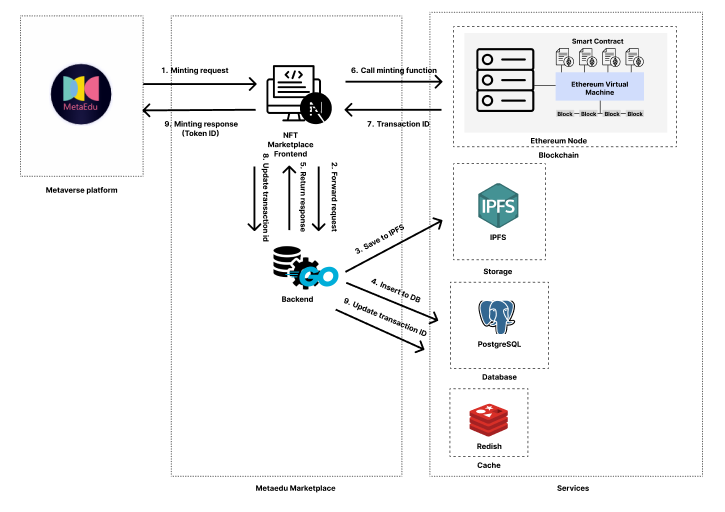
\includegraphics[width=\columnwidth,height=8cm]{gambar/img-integration-minting.png}
  % Keterangan gambar yang diinputkan
  \caption{\emph{Flow} pembagian kepemilikan NFT}
  % Label referensi dari gambar yang diinputkan
  \label{fig:Fractional}
\end{figure}

\subsection{\emph{Transaksi}}

\begin{figure} [H] \centering
  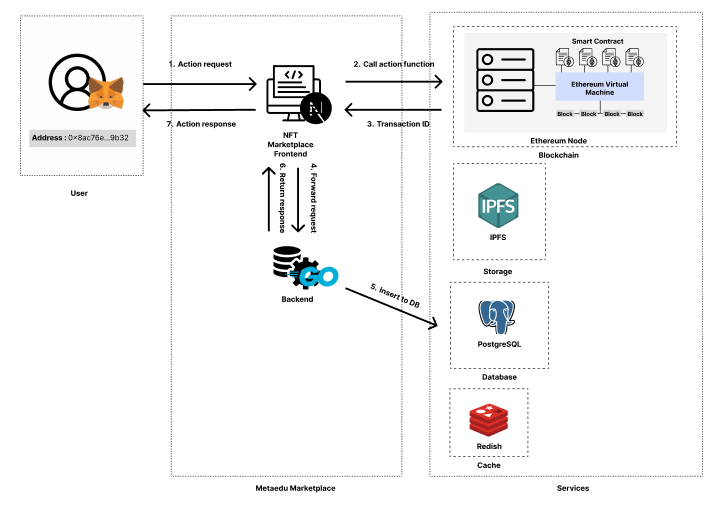
\includegraphics[scale=0.6]{gambar/img-integration-action.png}
  \caption{\emph{Flow} transaksi}
  \label{fig:ActionIntegration}
\end{figure}

Setelah melakukan proses \emph{minting} maka pengguna dapat melakukan transaksi berupa pembelian, peminjaman, ataupun pembagian kepemilikan terhadap \emph{NFT} baik antar pengguna maupun pengguna dengan \emph{platform} yang melakukan \emph{minting}.

\subsubsection{\emph{Fetching}}

\begin{figure} [H] \centering
  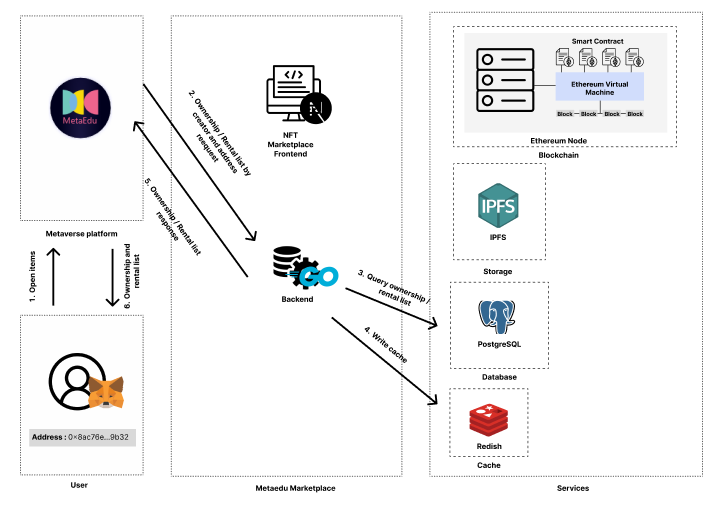
\includegraphics[scale=0.6]{gambar/img-integration-fetching.png}
  \caption{\emph{Flow fetching data}}
  \label{fig:FetchingIntegration}
\end{figure}

Tahap terakhir adalah proses \emph{fetching data}. Proses ini bertujuan supaya data \emph{NFT} yang di perjual belikan, disewakan, atau bahkan dibagikan kepemilikan dapat sinkron dengan \emph{platform metaverse}. Untuk melakukan hal tersebut pengguna platform yang terhubung dengan \emph{Wallet} memiliki \emph{Address}. Data berupa Address pengguna, ID creator token atau merupakan ID platform, dan ID token akan digunakan untuk mengakses \emph{endpoint} dari \emph{API} yang disediakan.

\begin{itemize}
  \item \emph{Endpoint} \emph{token} digunakan untuk memperoleh data \emph{NFT} yang di-\emph{minting} oleh \emph{platform} tersebut dengan menyertakan parameter \emph{id creator}.
   \item \emph{Endpoint} \emph{ownership} digunakan untuk memperoleh data kepemilikan atas suatu token dengan menyertakan parameter \emph{id token} atau data kepemilikan dari pengguna tertentu dengan menyertakan parameter \emph{Address} pengguna dan \emph{id creator}.
  \item \emph{Endpoint} \emph{rental} digunakan untuk memperoleh data peminjaman suatu \emph{token} dengan menyertakan parameter \emph{id token} atau data peminjaman pengguna dengan menyertakan parameter \emph{Address} pengguna dan \emph{id creator}.
  \item \emph{Endpoint} \emph{fraction} digunakan untuk memperoleh data mengenai pembagian kepemilikan suatu \emph{token} dengan menyertakan \emph{fraction token id} atau \emph{parent token id}
\end{itemize}

\section{Tools yang digunakan}

Dalam pengembangan \emph{NFT Marketplace} ini sesuai dengan arsitektu dan \emph{flow} yang dijelaskan sebelumnya diperlukan beberapa \emph{Software} dan \emph{Tools} dalam pengerjaannya. Dari sisi pengembangan \emph{Blockchain}-nya sendiri \emph{Software} yang digunakan adalah \emph{Solidity}, \emph{Hardhat}, \emph{Ehernal}, dan Metamask. Selain \emph{Blockchain} sendiri dibagi menjadi dua yaitu \emph{Frontend} dan \emph{Backend}. Pada sisi \emph{Frontend} yang menjadi tampilan muka dan tempat user berinteraksi adalah \emph{NextJS}, \emph{Typescript}, dan \emph{AntDesign}. Sedangkan pada sisi \emph{Backend} adalah \emph{Golang}, \emph{PostgreSQL}, \emph{Docker}, dan \emph{Redish}.

\begin{longtable}{|c|c|c|}
  \caption{\emph{Software} dan \emph{Tools} yang digunakan}
  \label{tb:EnergiKecepatan}                                   \\
  \hline
  \rowcolor[HTML]{C0C0C0}
  \textbf{\emph{Software/Tools}} & \textbf{Fungsi} \\
  \hline
  Solidity            & Bahasa pemrograman untuk mengembangkan \emph{smart contract}                                        \\
  Hardhat             & Simulasi \emph{blockchain} pada \emph{environment} lokal                                            \\
  Ethernal            & Melacak informasi pada \emph{blockchain}                                                            \\
  Metamask            & Sebagai \emph{Wallet} yang digunakan dalam bertransaksi                                             \\
  Golang              & Bahasa pemrograman untuk mengembangkan \emph{backend}                                               \\
  Redish              & Menyimpan \emph{cache}                                                                              \\
  PostgreSQL          & Menyimpan data-data                                                                                 \\
  Docker              & Memudahkan dalam melakukan proses \emph{setup} dan \emph{deployment}                                \\
  NextJS              & \emph{Framework} yang digunakan untuk mengembangkan \emph{frontend}                                 \\
  Typescript          & Bahasa pemrograman yang digunakan pada sisi \emph{frontend}                                         \\
  AntDesign           & \emph{Library} yang menyediakan berbagai komponen yang diperlukan pada \emph{frontend}              \\
  \hline
\end{longtable}

\subsection{\emph{Solidity}}

\emph{Solidity} merupakan bahasa pemrograman yang digunakan untuk mengembangkan \emph{smart contract} pada \emph{blockchain} \emph{Ethereum}. \emph{Solidity} termasuk ke dalam kategori \emph{multi bracket language}, artinya dibangun dengan beberapa bahasa pemrograman lain seperti C++, \emph{Python}, dan \emph{Javascript}, dan ditujukan supaya dapat berjalan pada \emph{EVM}. \emph{Smart contract} yang dibangun menggunakan \emph{Solidity} akan melakukan penyimpanan data dan pengiriman \emph{Ether} dari \emph{EOA} ke \emph{smart contract} maupun dari \emph{smart contract} ke EOA. 

\subsection{\emph{Hardhat}}

\emph{Hardhat} adalah lingkungan pengembangan \emph{Blockchain Ethereum}. \emph{Hardhat} mampu membuat dan mensimulasikan jaringan \emph{Ethereum} sehingga pengembang dapat mengembangkan \emph{Smart Contract} pada \emph{environment} lokalnya measing-masing. \emph{Software} ini juga akan membantu pengembang dalam \emph{compiling}, \emph{debugging}, \emph{deploying}, dan \emph{testing} pada \emph{Blockchain Ethereum}.
\begin{figure}[!h]
\centering 
  % Nama dari file gambar yang diinputkan
  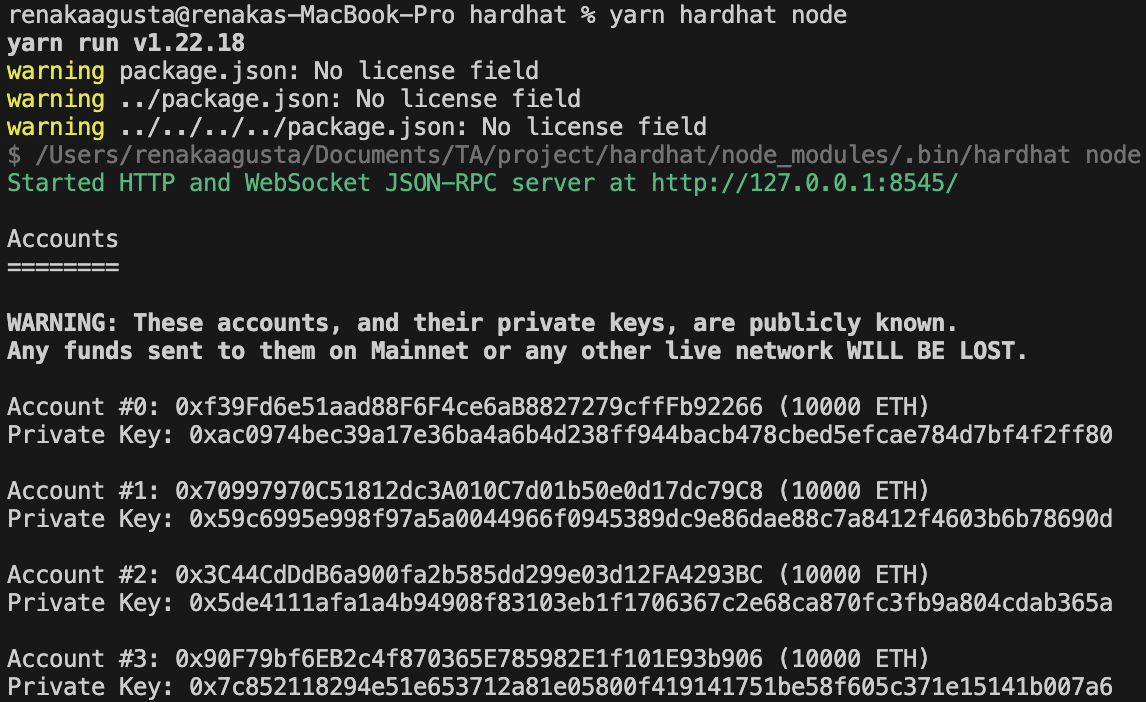
\includegraphics[scale=0.6]{gambar/img-hardhat.png}
  % Keterangan gambar yang diinputkan
  \caption{\emph{Hardhat}}
  % Label referensi dari gambar yang diinputkan
  \label{fig:Hardhat}
\end{figure}

\subsection{\emph{Ethernal}}

\emph{Ethernal} adalah \emph{Software Open Source} yang digunakan sebagai \emph{Blockchain Explorer} pada \emph{Blockchain Ethereum}. \emph{Block Explorer} membantu pengguna atau siapapun yang ingin mencari atau melacak informasi pada \emph{Blockchain} seperti transaksi, \emph{event}, akun, \emph{address}, dan sebagainya. Selain itu \emph{Ethernal} juga mendukung tampilan antarmuka dalam melakukan interaksi dengan \emph{Smart Contract} secara mudah. \emph{Software} ini juga tersedia sebagai \emph{plugin} dari \emph{hardhat} sehingga bagi pengembang yang telah menggunakan \emph{Hardhat} hanya perlu menambahkan \emph{plugin Ethernal} dan melakukan beberapa konfigurasi. Jika konfigurasi telah dilakukan, ketika proses \emph{compiling} dan \emph{deployment} \emph{ABI} akan diunggah ke \emph{Ethernal}.

\begin{figure}[H] 
  \centering
    % Nama dari file gambar yang diinputkan
    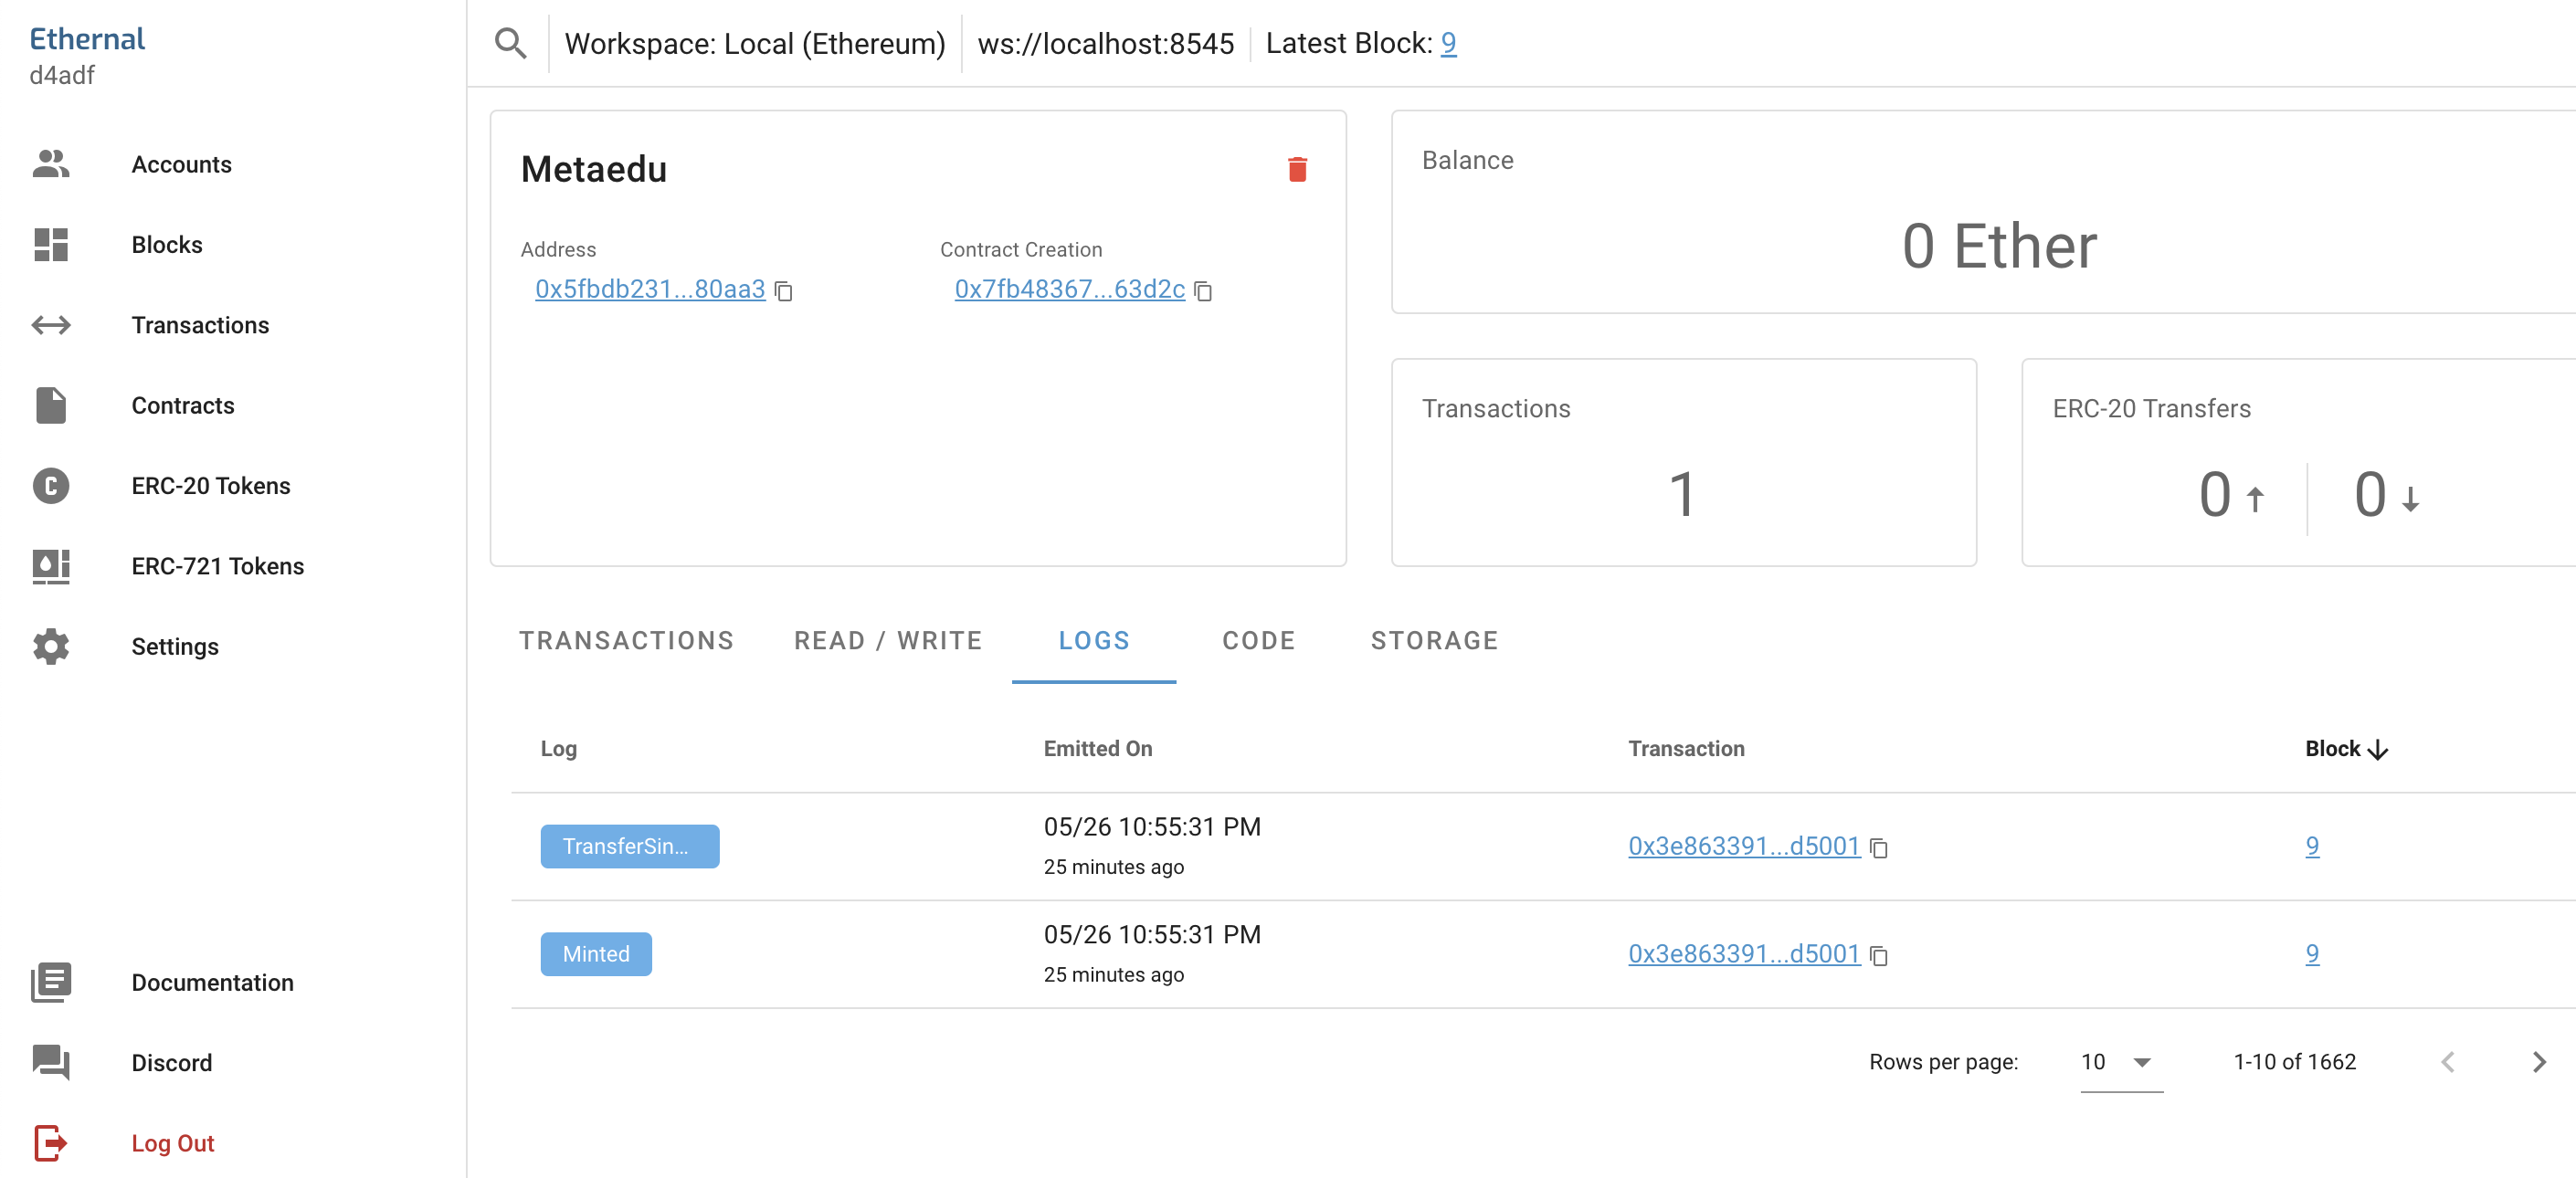
\includegraphics[scale=0.3]{gambar/img-ethernal.png}
    % Keterangan gambar yang diinputkan
    \caption{\emph{Ethernal}}
    % Label referensi dari gambar yang diinputkan
    \label{fig:Ethernal}
  \end{figure}

\subsection{\emph{Metamask}}

\emph{Metamask} adalah \emph{cold wallet} yang digunakan dalam melakukan menyimpan \emph{token}, bertransaksi dengan pengguna lain, dan berinteraksi dengan \emph{Smart Contract}. \emph{Metamask} hadir sebagai sebuah \emph{Extension} pada \emph{Browser}. Dengan menggunakan \emph{Metamask} pengguna tidak perlu memasukan \emph{Private key} setiap melakukan transaksi baik ketika membuat, menyimpan, ataupun menjual \emph{token}.

\begin{figure} [H] 
  \centering
  % Nama dari file gambar yang diinputkan
  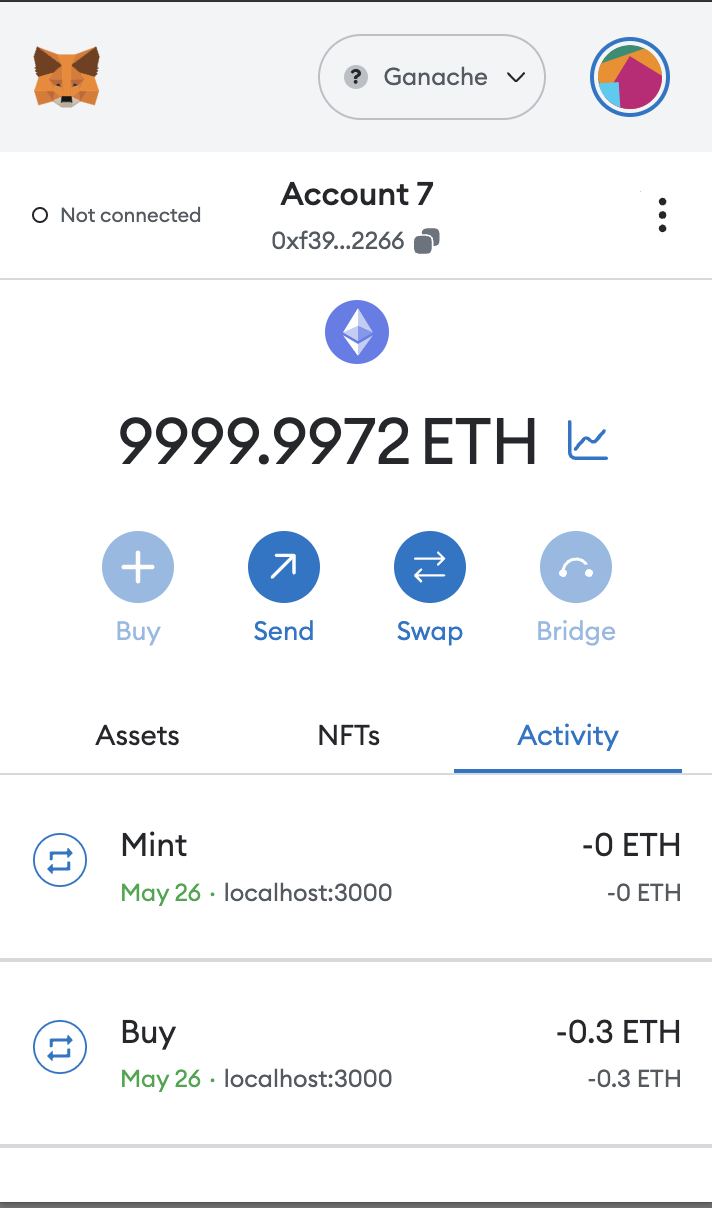
\includegraphics[scale=0.4]{gambar/img-metamask.png}
  % Keterangan gambar yang diinputkan
  \caption{\emph{Metamask}}
  % Label referensi dari gambar yang diinputkan
  \label{fig:Metamask}
\end{figure}

\section{Pengembangan \emph{Smart Contract}} 

Pada \emph{project} ini \emph{Smart Contract} dibuat untuk menjembatani dan memperoses \emph{request} dari yang dihasilkan dari interaksi pengguna ke jaringan \emph{Blockchain}. Untuk membuat \emph{NFT Marketplace} sesuai dengan \emph{Flow} yang telah ditentukan sebelumnya maka diperlukan \emph{Smart Contract} yang digunakan akan berisi berbagai \emph{variable} yang digunakan untuk menampung data-data yang dibutuhkan, \emph{function} untuk memproses data sesuai alur yang ditentukan, \emph{modifier} untuk memvalidasi parameter yang dikirim, serta \emph{event} yang digunakan untuk merekam suatu aktivitas yang terjadi pada \emph{smart contract}. 

\subsection{\emph{Variable}}

\emph{Variable} pada \emph{smart contract} berfungsi menyimpan data-data untuk kemudian diolah oleh \emph{function}. pada \emph{smart contract} ini ada beberapa \emph{variable} yang dibuat.

% Contoh pembuatan potongan kode
\begin{lstlisting}[
  language=C++,
  caption={Variable},
  label={lst:variable},
  basicstyle=\tiny,
]
  address public ownerAddress;

  Counters.Counter private tokenIds;
  mapping(uint256 => string) private uris;
  mapping(uint256 => uint256) private supplies;
  
  mapping(uint256 => mapping(address => ItemForSale)) public itemsForSale;
  mapping(uint256 => mapping(address => ItemForRent)) public itemsForRent;
  
  mapping(uint256 => uint256) private fractionsMapping;
\end{lstlisting}

\begin{itemize}
  \item \emph{ownerAddress} digunakan untuk menyimpan \emph{address} dari \emph{owner smart contract}. \emph{Variable} ini di \emph{set} ketika \emph{smart contract} di \emph{deploy}.
  \item \emph{tokenIds} digunakan untuk menyimpan index \emph{token} terakhir yang di-\emph{minting}.
  \item \emph{uris} digunakan untuk menyimpan data \emph{uri} dari setiap \emph{token} yang di-\emph{minting} dalam \emph{smart contract}. 
  \item \emph{supplies} digunakan untuk menyimpan data \emph{supply} atau jumlah dari masing-masing \emph{token}.
  \item \emph{itemsForSale} digunakan untuk menyimpan data \emph{token} yang dapat diperjual belikan.
  \item \emph{itemsForRent} digunakan untuk menyimpan data \emph{token} yang dapat disewakan.
\end{itemize}

\subsection{\emph{Event}}

\emph{Event} adalah suatu aktivitas tertentu terekam dalam \emph{Smart Contract}. Setiap pengembang dapat membuat \emph{Event}-nya sesuai dengan kebutuhan. Nantinya \emph{Event}-\emph{Event} ini dapat dilacak dan dilihat secara publik. 

% Contoh pembuatan potongan kode
\begin{lstlisting}[
  language=C++,
  caption={Program halo dunia.},
  label={lst:halodunia},
  basicstyle=\tiny,
]
event Minted(
  uint256 indexed tokenId,
  string uri,
  address indexed owner,
  address indexed nftAddress,
  uint256 supply
);
event ShareOwnership(
  uint256 indexed tokenId,
  address indexed owner,
  uint256 supply
);
event ItemAddedForSale(
  uint256 tokenId,
  address owner,
  uint256 supply,
  uint256 price
);
event ItemAddedForRent(
  uint256 tokenId,
  address owner,
  uint256 supply,
  uint256 price
);
event ItemBuy(
  address buyer,
  address seller,
  uint256 tokenId,
  uint256 price
); 
event ItemRent(
  address user,
  address owner,
  uint256 tokenId,
  uint256 price,
  uint256 day
); 
\end{lstlisting}

\begin{itemize}
  \item \emph{Minted} adalah aktivitas yang digunakan untuk menandai bahwa terdapat \emph{token} baru yang di-\emph{minting}.
  \item \emph{ShareOwnership} adalah aktivitas yang digunakan untuk menanandai bahwa terdapat \emph{NFT} yang di-\emph{fraction}.
  \item \emph{ItemAddedForSale} adalah aktivitas yang digunakan untuk menandai bahwa terdapat \emph{token} yang dapat diperjual belikan.
  \item \emph{ItemAddedForRent} adalah aktivitas yang digunakan untuk menandai bahwa terdapat \emph{token} yang dapat disewakan.
  \item \emph{ItemBuy} adalah aktivitas yang digunakan untuk menandai bahwa terdapat \emph{token} yang dibeli. 
  \item \emph{ItemRent} adalah aktivitas yang digunakan untuk menandadi bahwa terdapat \emph{token} yang disewa.
\end{itemize}

\subsection{\emph{Modifier}}

\emph{Modifier} adalah \emph{block code} yang digunakan untuk memvalidasi parameter yang diberikan dalam pemanggilan \emph{function} tertentu. \emph{Modifier} memastikan bahwa segala parameter telah valid sebelum diproses oleh suatu \emph{function}.

% Contoh pembuatan potongan kode
\begin{lstlisting}[
  language=C++,
  caption={Modifier},
  label={lst:modifier},
  basicstyle=\tiny,
]
modifier ItemIsNonFungible(uint256 _tokenId) {
  require(supplies[_tokenId] == 1, "Token is fungible");
}

modifier ItemIsAvailableForBuy(uint256 _tokenId, address _seller) {
  require(
      itemsForSale[_tokenId][_seller].isSold == false,
      "Token is sold"
  );
}

modifier ItemIsAvailableForRent(
  uint256 _tokenId,
  address _seller,
  uint256 datetime
) {
  require(
      itemsForRent[_tokenId][_seller].expirationTime <= datetime ||
          itemsForRent[_tokenId][_seller].expirationTime == 0,
      "Token is rented"
  );
}

modifier BuyerIsValid(uint256 _tokenId, address _seller) {
  require(msg.sender != _seller, "Buyer is not valid");
}

modifier UserIsValid(uint256 _tokenId, address _owner) {
  require(msg.sender != _owner, "Buyer is not valid");
}

modifier AmountForBuyIsValid(uint256 _price) {
  require(msg.value >= _price * 1000000000000, "Amount is not valid");
}

modifier AmountForRentIsValid(uint256 _price) {
  require(msg.value >= _price * 1000000000000, "Amount is not valid");
}

modifier ItemIsAvailableForSale(uint256 _tokenId, uint256 _supply) {
  uint256 itemSupply = balanceOf(msg.sender, _tokenId);
  uint256 sellItemSupply = itemsForSale[_tokenId][msg.sender].supply;
  uint256 availableItemSupply = itemSupply - sellItemSupply;
  require(
      availableItemSupply > _supply,
      "Item is not available for sale"
  );
}

modifier ItemIsNotInRentalPeriod(
  uint256 _tokenId,
  address _owner,
  uint256 _datetime
) {
  require(
      itemsForRent[_tokenId][_owner].expirationTime < _datetime,
      "Item is in rental period"
  );
}
\end{lstlisting}

\begin{itemize}
  \item \emph{ItemIsNonFungible} digunakan untuk memvalidasi bahwa \emph{token} merupakan \emph{NFT}.
  \item \emph{ItemIsAvailableForBuy} digunakan untuk memvalidasi bahwa \emph{token} dapat dibeli.
  \item \emph{ItemIsAvailableForRent} digunakan untuk memvalidasi bahwa \emph{token} dapat disewa.
  \item \emph{BuyerIsValid} digunakan untuk memvalidasi bahwa pembeli memiliki \emph{address} yang berbeda dengan \emph{seller} \emph{token}.
  \item \emph{UserIsValid} digunakan untuk memvalidasi bahwa penyewa memiliki \emph{address} yang berbeda dengan \emph{owner} \emph{token}.
  \item \emph{AmountForBuyIsValid} digunakan untuk memvalidasi bahwa \emph{ether} yang dikirim sesuai dengan harga dari \emph{token} yang dibeli.
  \item \emph{AmountForRentIsValid} digunakan untuk memvalidasi bahwa \emph{ether} yang dikirim sesuai dengan harga sewa dari \emph{token}.
  \item \emph{ItemIsNotInRentalperiod} digunakan untuk memvalidasi bahwa \emph{token} tidak sedang dalam masa penyewaan.
\end{itemize}

\subsection{\emph{Function}}

\emph{Function} adalah \emph{block code} berisi \emph{logic} untuk memperoses data sesuai dengan \emph{business logic} yang telah ditentutkan. \emph{Function}-\emph{function} utama dalam \emph{smart contract} yang dikembangkan diantaranya adalah \emph{mint}, \emph{putItemForSale}, \emph{putItemForRent}, \emph{buy}, \emph{rent}, \emph{shareOwnership}

\subsubsection{\emph{Mint}}

% Contoh pembuatan potongan kode
\begin{lstlisting}[
  language=C++,
  caption={Mint},
  label={lst:mint},
  basicstyle=\tiny,
]
function mint(
  uint256 _supply,
  string memory _uri
) public {
  tokenIds.increment();
  uint256 tokenId = tokenIds.current();
  _mint(msg.sender, tokenId, _supply, "");
  uris[tokenId] = _uri;
  supplies[tokenId] = _supply;
  emit Minted(tokenId, _uri, msg.sender, address(this), _supply);
}
\end{lstlisting}

\emph{Function} \emph{mint} digunakan untuk mendaftarkan \emph{token} baru dimana proses ini biasa dikenal sebagai \emph{minting}. Parameter pada funsi ini adalah \emph{supply} yang berisi jumlah \emph{token} yang beredar. Jika nilai \emph{supply} yang dikirimkan adalah 1 maka \emph{token} tersebut adalah NFT sebaliknya jika lebih dari 1 maka \emph{token} tersebut adalah \emph{token fungible}.

\subsubsection{\emph{PutItemForSale}}

% Contoh pembuatan potongan kode
\begin{lstlisting}[
  language=C++,
  caption={Mint},
  label={lst:mint},
  basicstyle=\tiny,
]
function putItemForSale(
  uint256 _tokenId,
  uint256 _price,
  uint256 _supply,
  uint256 _datetime
)
  external
  ItemIsNotInRentalPeriod(_tokenId, msg.sender, _datetime)
  OwnerIsValid(_tokenId)
{
  itemsForSale[_tokenId][msg.sender] = ItemForSale({
      tokenId: _tokenId,
      supply: _supply,
      seller: payable(msg.sender),
      price: _price,
      isSold: false
  });
  emit ItemAddedForSale(_tokenId, msg.sender, _supply, _price);
}
\end{lstlisting}

\emph{Function} \emph{putItemForSale} supaya pemilik \emph{token} dapat menjual \emph{token} yang dimiliki. \emph{Function} ini perlu dipanggil apabila pemilik menghendaki untuk menjual dikarenakan \emph{token} yang baru saja di-\emph{minting} tidak dapat langsung diperjual belikan.

\subsubsection{\emph{PutItemForRent}}

% Contoh pembuatan potongan kode
\begin{lstlisting}[
  language=C++,
  caption={Rent},
  label={lst:rent},
  basicstyle=\tiny,
]
function putItemForRent(
  uint256 _tokenId,
  uint256 _price,
  uint256 _supply,
  uint256 _datetime
)
  external
  ItemIsNotInRentalPeriod(_tokenId, msg.sender, _datetime)
  OwnerIsValid(_tokenId)
  ItemIsNonFungible(_tokenId)
{
  itemsForRent[_tokenId][msg.sender] = ItemForRent({
      tokenId: _tokenId,
      supply: _supply,
      owner: payable(msg.sender),
      user: msg.sender,
      price: _price,
      expirationTime: 0
  });
  emit ItemAddedForRent(_tokenId, msg.sender, _supply, _price);
}
\end{lstlisting}

\emph{Function} \emph{putItemForRent} supaya pemilik \emph{token} dapat menyewakan \emph{token} yang dimiliki. \emph{Function} ini perlu dipanggil apabila pemilik menghendaki untuk menyewakan \emph{token}-nya dikarenakan \emph{token} yang baru saja di-\emph{minting} tidak dapat langsung disewakan.

\subsubsection{\emph{Buy}}

% Contoh pembuatan potongan kode
\begin{lstlisting}[
  language=C++,
  caption={Buy},
  label={lst:buy},
  basicstyle=\tiny,
]
function buy(
  uint256 _tokenId,
  uint256 _quantity,
  address payable _seller,
  uint256 _datetime
)
  external
  payable
  BuyerIsValid(_tokenId, _seller)
  ItemIsNotInRentalPeriod(_tokenId, _seller, _datetime)
  AmountForBuyIsValid(itemsForSale[_tokenId][_seller].price)
  ItemIsAvailableForBuy(_tokenId, _seller)
{
  safeTransferFrom(_seller, msg.sender, _tokenId, _quantity, "0x0");
  itemsForSale[_tokenId][_seller].isSold = true;
  _seller.transfer(msg.value);
}
\end{lstlisting}

\emph{Function} \emph{buy} digunakan untuk memproses \emph{request}  pembelian \emph{token} oleh user.

\subsubsection{\emph{Rent}}

% Contoh pembuatan potongan kode
\begin{lstlisting}[
  language=C++,
  caption={Rent},
  label={lst:rent},
  basicstyle=\tiny,
]
function rent(
  uint256 _tokenId,
  uint256 _day,
  address payable _owner,
  uint256 _datetime
)
  external
  payable
  ItemIsNotInRentalPeriod(_tokenId, _owner, _datetime)
  UserIsValid(_tokenId, _owner)
  AmountForRentIsValid(itemsForRent[_tokenId][_owner].price * _day)
  ItemIsAvailableForRent(_tokenId, _owner, _datetime)
{
  itemsForRent[_tokenId][_owner].expirationTime = (_day * 86400000)+_datetime;
  itemsForRent[_tokenId][_owner].user = msg.sender;
  _owner.transfer(msg.value);
}
\end{lstlisting}

\emph{Function} \emph{rent} digunakan untuk memproses \emph{request} penyewaan \emph{token} yang belum di-\emph{fraction} oleh \emph{owner} dari \emph{token} tersebut.

\subsubsection{\emph{RentFraction}}

% Contoh pembuatan potongan kode
\begin{lstlisting}[
  language=C++,
  caption={RentFraction},
  label={lst:rentFraction},
  basicstyle=\tiny,
]
function rentFraction(
        uint256 _tokenId,
        uint256 _day,
        address payable[] memory _ownerList,
        uint256[] memory _shareList,
        uint256 _datetime
    )
        external
        payable
        ItemIsNotInRentalPeriod(_tokenId, ownerAddress, _datetime)
        UserIsValid(_tokenId, ownerAddress)
        AmountForRentIsValid(itemsForRent[_tokenId][ownerAddress].price * _day)
        ItemIsAvailableForRent(_tokenId, ownerAddress, _datetime)
    {
        ItemForRent memory itemForRent = itemsForRent[_tokenId][ownerAddress];
        itemForRent.expirationTime = (_day * 86400000) + _datetime;
        itemForRent.user = msg.sender;
        for (uint256 i = 0; i < _ownerList.length; i++) {
            if (
                balanceOf(_ownerList[i], fractionsMapping[_tokenId]) ==
                _shareList[i]
            ) {
                _ownerList[i].transfer(
                    (msg.value * _shareList[i]) /
                        supplies[fractionsMapping[_tokenId]]
                );
            }
        }
    }
\end{lstlisting}

\emph{Function} \emph{rentFraction} digunakan untuk memproses \emph{request} penyewaan \emph{token} yang telah di-\emph{fraction} oleh \emph{owner} dari \emph{token} tersebut. Perbedaan dari \emph{function} \emph{rent} sebelumnya adalah \emph{function} ini membagikan \emph{ether} yang dikirim kepada seluruh \emph{address} yang memiliki \emph{token} hasil \emph{fraction} sebanding dengan jumlah kepemilikannya.

\section{Penyiapan \emph{Database}}

\emph{Database} adalah kumpulan dari data-data yang dikelola berdasarkan sedemikan rupa berdasarkan ketentuan tertentu. Pada \emph{project} \emph{NFT Marketplace} ini digunakan untuk menyimpan berbagai data seperti data \emph{user}, \emph{token}, \emph{ownership}, \emph{rental}, \emph{fraction}, dan \emph{transaction}. Data-data ini juga disimpan pada \emph{Blockchain}, akan tetapi untuk mayoritas proses pengambilan data akan diperoleh dari \emph{database} supaya dapat memberikan kecepatan pemrosesan yang lebih cepat. Database yang digunakan adalah \emph{PostgreSQL} hal ini dikarenakan \emph{PostgreSQL} mampu memberikan keamanan dalam pemprosesan suatu transaksi dikarenakan telah \emph{comply} dengan prinsip \emph{ACID} (\emph{Atomicity, Consistency, Isolation, and Durability}). Hal ini menjadi penting untuk menghindari kerusakan data akibat adanya kegagalan sistem ketika transaksi antar \emph{user} sedang diproses. Selain itu, walaupun PostgreSQL merupakan \emph{SQL} (Structured query language), \emph{database} ini juga mampu menyimpan data yang \emph{semi-unstructured} seperti \emph{JSON} \emph{(JavaScript Object Notation)} yang digunakan untuk menyimpan \emph{metadata} \emph{token}.

\begin{figure} [H] \centering
  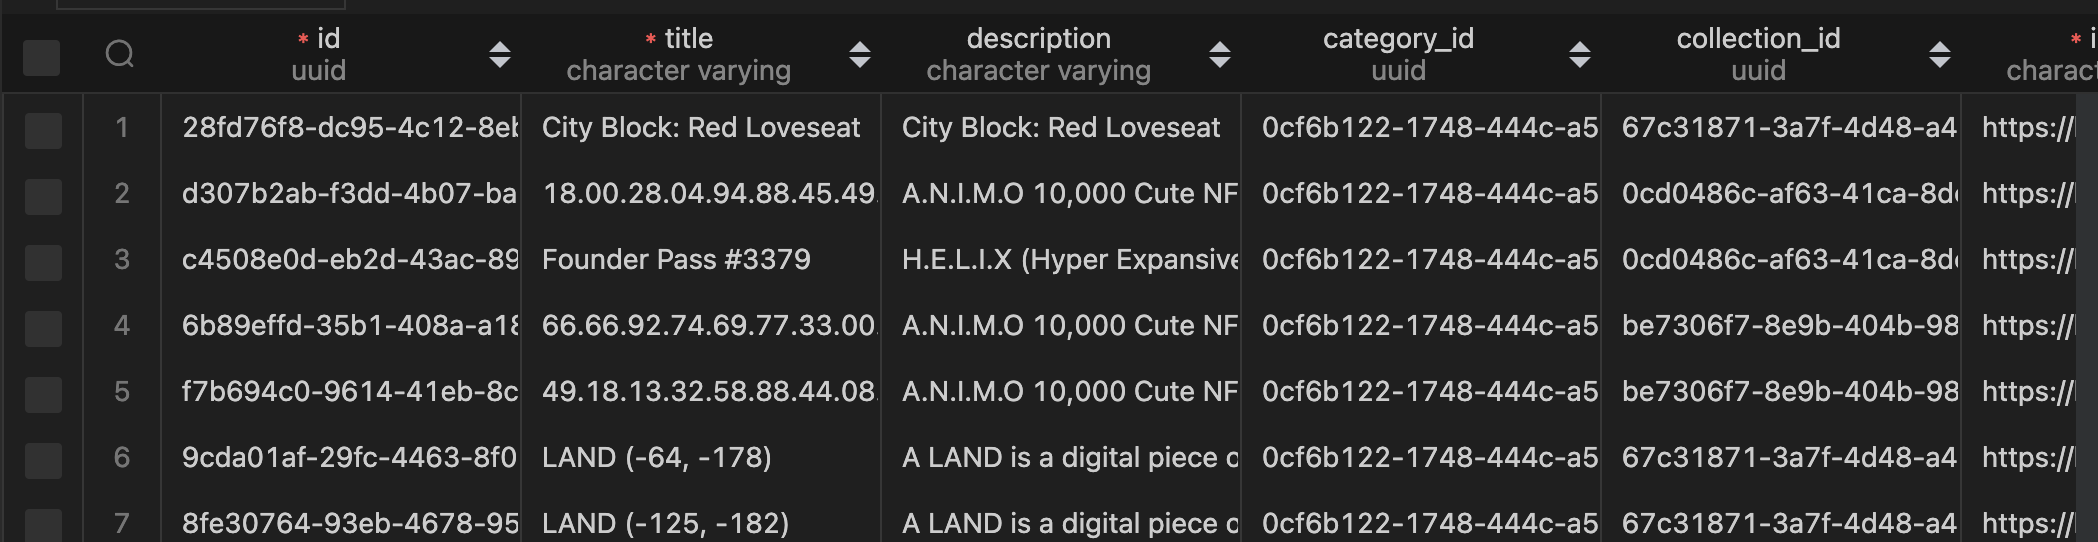
\includegraphics[scale=0.35]{gambar/img-table-tokens.png}
  \caption{Tabel \emph{token}}
  \label{fig:TokenTable}
\end{figure}

Digunakan untuk menyimpan data \emph{token} seperti nama, deskripsi, kategori, koleksi dan lainnya terkait dengan suatu \emph{token}.

\begin{figure} [H] \centering
  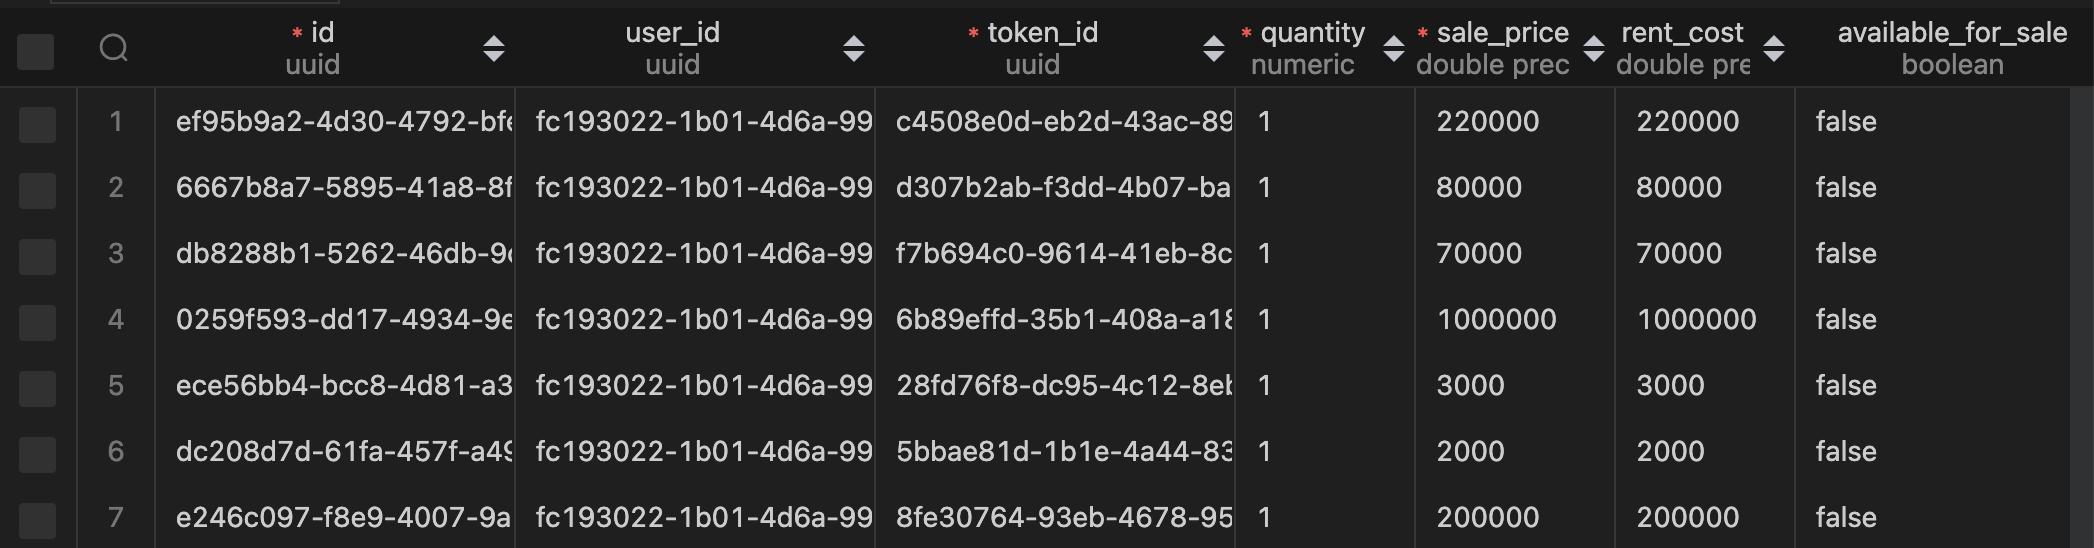
\includegraphics[scale=0.35]{gambar/img-table-ownerships.png}
  \caption{Tabel \emph{ownerships} }
  \label{fig:OwnershipTable}
\end{figure}

Digunakan untuk menyimpan data kepemilikan suatu token oleh pengguna meliputi id token, id pengguna, jumlah kepemilikan, status penjualan, dan status penyewaan.

\begin{figure} [H] \centering
  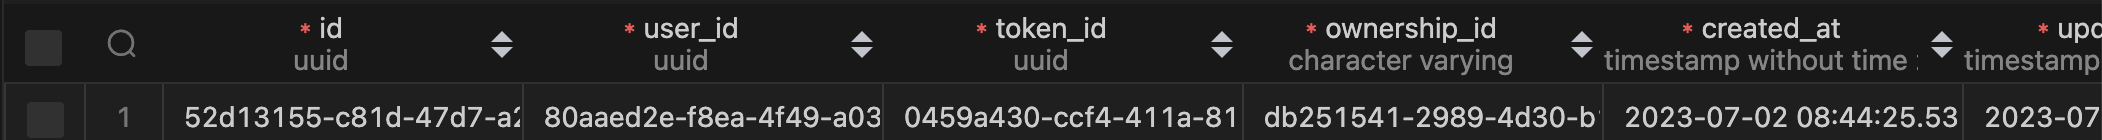
\includegraphics[scale=0.35]{gambar/img-table-rentals.png}
  \caption{Tabel \emph{rentals}}
  \label{fig:OwnershipTable}
\end{figure}

Digunakan untuk menyimpan data penyewaan suatu token oleh pengguna meliputi id token, id kepemilikan, id pengguna, dan lama penyewaan.

\begin{figure} [H] \centering
  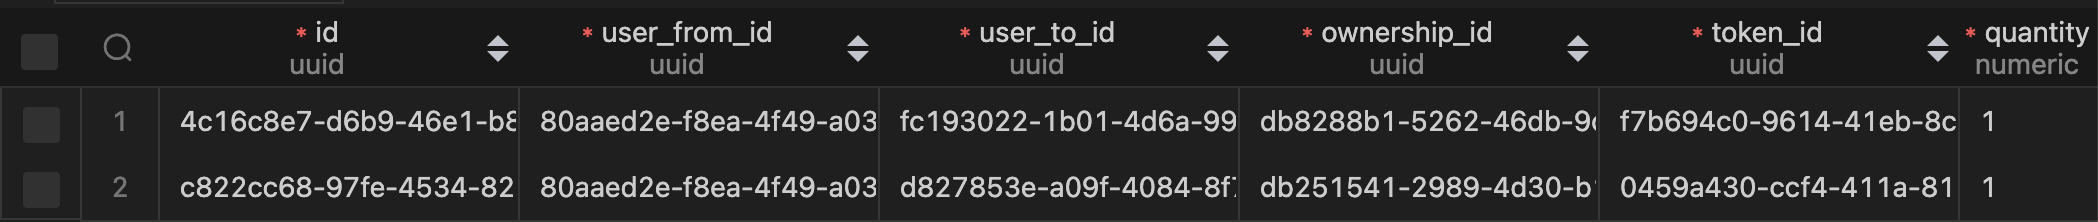
\includegraphics[scale=0.35]{gambar/img-table-transactions.png}
  \caption{Tabel \emph{rentals}}
  \label{fig:TransactionsTable}
\end{figure}

Digunakan untuk menyimpan data transaksi baik penjualan maupun penyewaan yang meliputi id pembeli, id penjual, id token, dan jumlah token yang dijual.

\begin{figure} [H] \centering
  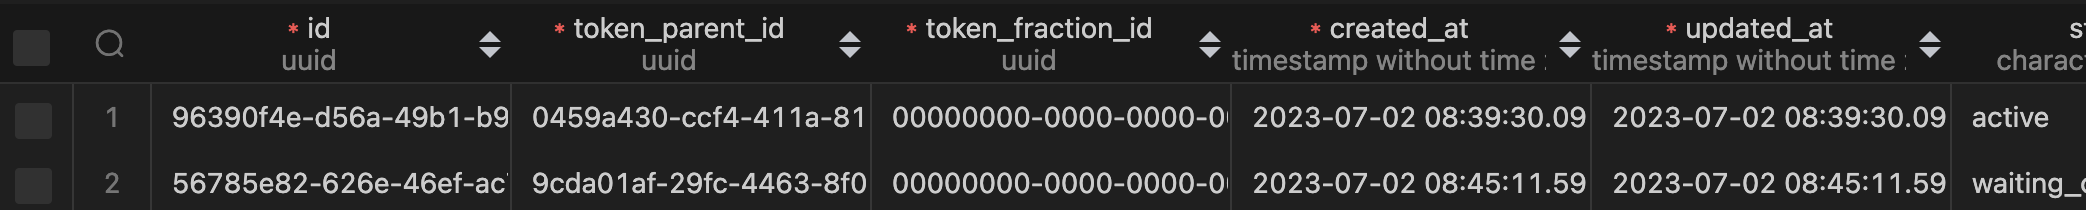
\includegraphics[scale=0.35]{gambar/img-table-fractions.png}
  \caption{Tabel \emph{fractions}}
  \label{fig:FractionsTable}
\end{figure}

Digunakan untuk menyimpan data \emph{fractionilalizations} suatu token hasil proses \emph{share ownership} oleh pengguna meliputi id token asal, id token pencahan, dan id pengguna.

\section{Pengembangan \emph{Back End}} 

\emph{Back End} adalah bagian dari aplikasi yang tidak terlihat oleh pengguna yang memproses seluruh data ketika \emph{request} dikirimkan oleh \emph{user}. Aplikasi \emph{Back End} dikembangkan menggunakan bahasa pemrograman \emph{Golang}. \emph{Golang} dipilih dikarenakan memiliki performat yang lebih cepat dari banyak bahasa pemrograman lain. Hal tersebut dikarenakan \emph{Golang} adalah \emph{Compiled language} bukan \emph{Interpreted language} sehingga dapat langsung dibaca oleh mesin. Selain itu \emph{Golang} juga memiliki fitur \emph{multithread} sehingga akan memaksimalkan potensi dari \emph{Server} yang digunakan. Aplikasi \emph{Back End} akan mengambil data dari \emph{Database} yang dalam hal ini adalah \emph{PostgreSQL} dan juga \emph{Redish} sebagai tempat penyimpanan \emph{Cache}. Ketika data yang butuhkan oleh \emph{user} tidak ada di \emph{Redish} maka \emph{aplikasi} akan mengambil data dari \emph{Database} kemudian data tersebut aplikasi melakukan proses \emph{write} \emph{cache} pada \emph{Redis} sehingga jika ada \emph{user} lain memerlukan data yang sama tidak perlu mengambil data kembali dari \emph{Database}.

Aplikasi \emph{Back End} yang dikembangkan berupa \emph{API} (\emph{Application Programming Interdace}) yang nantinya akan diakses oleh \emph{frontend} dan \emph{platform metaverse} melalui protokol \emph{HTTP/HTTPS}. 

\section{Pengembangan \emph{Front End}} 

\emph{Front End} adalah bagian dari aplikasi yang terlihat dan menjadi tempat berinteraksi \emph{user}. Pada pengembangan \emph{project} \emph{NFT Marketplace} ini dipilih \emph{NextJS} sebagai \emph{framework}-nya. \emph{NextJS} dipilih dikarenakan memiliki fitur \emph{server side rendering}. Hal ini berarti \emph{Server} mampu menghasilkan \emph{HTML} untuk sebuah halaman dan mengirimkannya langsung kepada \emph{client}. Sebaliknya \emph{framework} lain layaknya \emph{ReactJS} mengirimkan \emph{Javascript} kepada \emph{Client} kemudian \emph{Client} sendiri lah yang akan memproses nya untuk memperoleh \emph{HTML}. Dengan fitur tersebut mampu meningkatkan aspek \emph{SEO} dari \emph{web} yang dikembangkan. Selain itu pengembangan aplikasi \emph{Front End} juga dikolaborasikan dengan \emph{framework} lain seperti \emph{tailwind} dan \emph{AntDesign} untuk memberikan tampilan yang lebih konsisten.  

